\begin{table}[tb]
    \centering 
    % latex table generated in R 4.4.1 by xtable 1.8-4 package
% Thu Oct 10 16:54:40 2024
\begin{tabular}{lllll}
  \hline
Slice & Var Bayes & Monte Carlo & Reg w/ FE & Reg w/o FE \\ 
  \hline
Threshold & 3 & ~ & ~ & ~ \\ 
  Delaware & 4 & 30 & ~ & ~ \\ 
  Restricted & 8 & 21 & 127 & 118 \\ 
  Critical & 11 & 51 & 30 & 22 \\ 
   \hline
\end{tabular}

    \caption{Counts of emergent clusters identified in data slices, as via posterior sampling.\label{tab:extant_clusters}}
\end{table}

In Section~\ref{sec:slosh} we described our criteria for narrowing the focus of our analysis,
    and specifically in Table~\ref{tab:datasets} we detailed the number of observations, and
    number of storm simulations, for the resulting datasets at each stage of this narrowing
    process.  In Table~\ref{tab:extant_clusters}, we detail the number of clusters that emerge
    in fitting our model to these datasets.  In all cases, for the Pitman-Yor process parameters,
    we used a concentration parameter $\eta = 0.1$, along with a discount parameter also of $0.1$.
    For any given model and dataset, the number of emergent clusters found was relatively robust 
    to our choice of parameters, for concentration within a range from \num{0.01}--\num{20}, and
    discount within a range \num{0.001}--\num{2}.  Higher values for both generally resulted in
    slightly more emergent clusters, but did not change the total number by more than \num{10} percent.
    Here we encounter an issue:  the model fitted via variational methods, and the model fitted 
    via MCMC methods, are nominally the same model, and should result in a similar number of 
    emergent clusters. That there is such a discrepancy is likely a weakness of the variational
    fitting process.  In the variational Bayes fitting method, we see the number of extant
    clusters fall significantly as the number of dimensions rises.  This behavior is predicted 
    by \cite{chandra2023}, which argues that as dimensionality increases, a BNP mixture model 
    will degenerate to one of two possible states: every observation falling into a single 
    cluster, or every cluster a singleton. We do not quite see that happen yet in the MCMC approach,
    where we see the number of extant clusters actually rise slightly between Delaware slice 
    and the Threshold slice.  However, the dimensionality of the threshold slice is approximately
    14.6 times that of the Delaware slice, and the number of simulations which meet the criteria
    for inclusion in the Threshold slice is approximately 1.4 times that of the Delaware slice.
    Taking into account the associated increase in data complexity between the two slices, we
    should see \emph{significantly more} clusters.  That we only see marginally more appears to
    indicate that the BNP mixture of projected gammas will eventually degenerate towards a 
    single cluster.
    \cite{chandra2023} suggests an amelioration of this behavior: to instead base the 
    BNP process on a lower-dimensional representation of the output space---suggesting 
    a factor analysis.  The regression model we have developed works in a similar manner, 
    representing an $S$-dimensional space using a $d$-dimensional vector.  In the regression
    models, we see the opposite problem occuring: there are too many clusters.  The Pitman-Yor
    process is accounting for the lack of information in $\bm{X}$, the regressors, by producing
    more clusters.  We see evidence to this interpretation by the addition of the random 
    effects.  By including random effects in the model specification, more information is 
    contained within the regressors, and thus a single cluster is able to represent slightly 
    more varied outcomes.  Thus, the number of emergent clusters is marginally reduced.

\begin{figure}[ht]
    \centering
    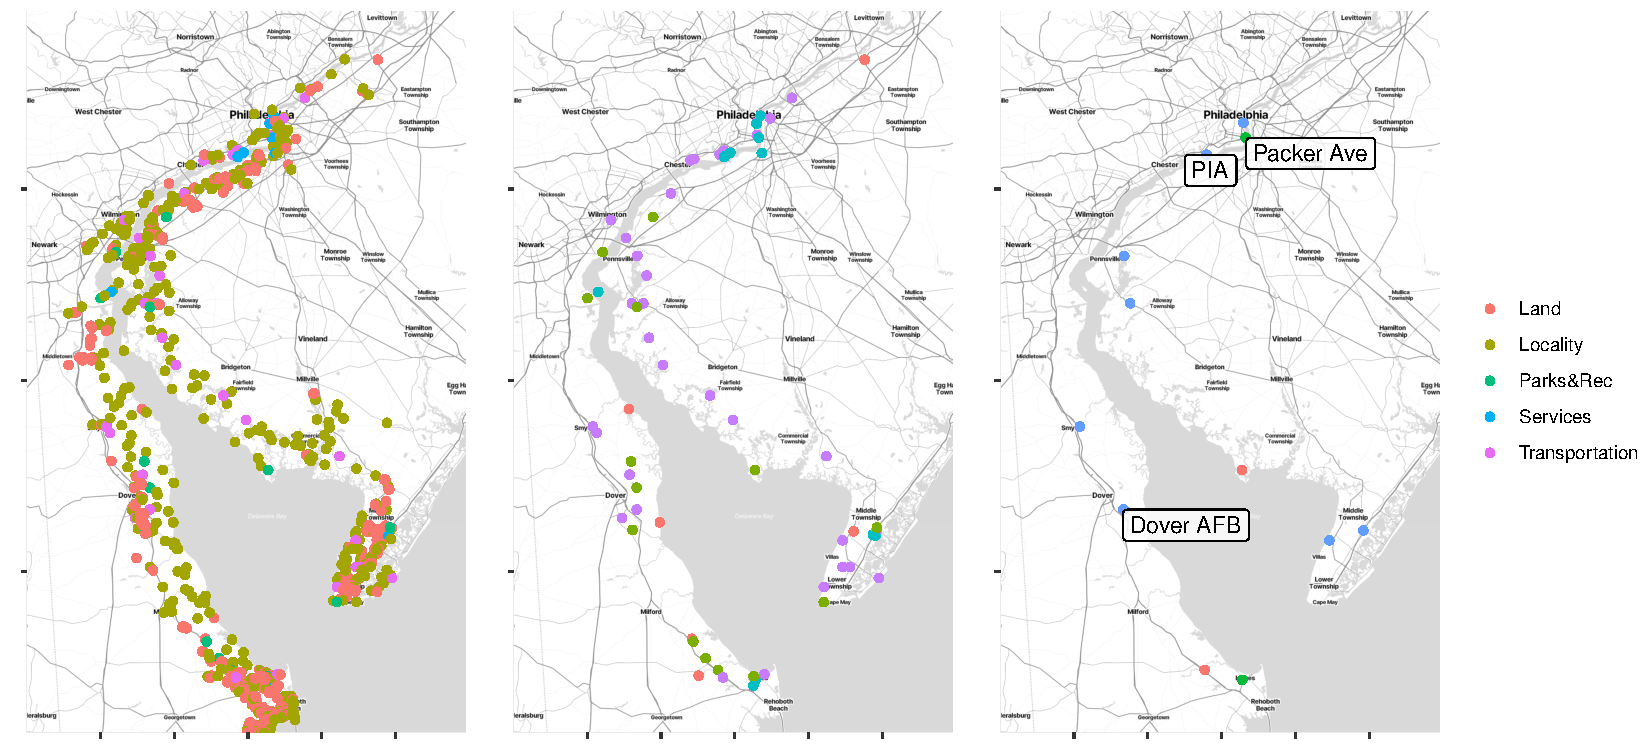
\includegraphics[width=0.99\linewidth]{./plots/delaware}
    \caption{Locations of identified sites in the \emph{Delaware} (left), 
    \emph{Restricted} (center), and \emph{Critical} (right) Slices.  
    Three locations of interest in further analysis have been specifically identified.
    \label{map:delawarebay}}
\end{figure}

Given the geographical focus inherent to the original data, we concentrate our primary
    analysis on Delaware Bay.  Figure~\ref{map:delawarebay} gives the locations of sites
    we identified, along with a classification of those sites.  The original feature class
    codes in the TIGER location data were sorted into five categories:  ``Land'' includes
    prominent land features, as well as some road features; ``Locality'' includes major road
    intersections, communities, or populated places; ``Parks\&Rec'' includes state and local
    parks, cemeteries, and places of worship; ``Services'' includes emergency services: police,
    fire, and medical services, and ``Transportation'' includes airports, heliports, ferry
    landings, and other major transportation infrastructure.  We identify within the data
    three locations which are of particular interest, for which significant inundation can
    can lead to catastrophic consequences.  Dover Air Force Base (Dover AFB) is a military
    installation on the South shore of the Delaware Bay, with a direct line of approach from 
    the ocean.  Philadelphia International Airport  (PIA) is a major airport, situated on the 
    bank of the Delaware River, near Philadelphia.   PIA is much further upstream relative to
    Dover AFB, and would require a storm to backflow the Delaware River a significant amount
    to reach it.  Packer Avenue Terminal is a major shipping hub, connecting transport ships to
    truck and rail transport services.  It is situated only slightly further upstream than PIA,
    so we would expect outcomes for these two locations to be strongly dependent.
    Inundation in any of these three locations could lead to significant negative consequences.
    \makenote{describe those consequences?}

\subsection{Assessing Model Fidelity\label{subsec:sloshfidelity}}

One difficulty with a high-dimensional model is evaluating its fidelity.  As we saw in 
    the simulation study, the relative rise in energy score between a bad modeling approach 
    and a good modelling approach shrinks as data complexity increases.  However, as we 
    saw in Table~\ref{tab:extant_clusters}, MCMC and what appears to be a similarly good 
    modelling approach yield very different outcomes.  This disconnect in assessment of 
    model fidelity using energy score as a criterion is related to the curse of dimensionality 
    in applications like $k$-nearest neighbor algorithms: as the number of dimensions 
    increases, the ratio in average distance between the nearest replicate, and farthest 
    replicate in a sample will tend to approach unity.  In this regard, distance, and metrics 
    based on distance will be fundamentally flawed in a high-dimensional setting.

As a partial amelioration of this issue, we can subjectively assess recovery of marginal 
    empirical CDF, by observing the marginal posterior predictive CDF for various locations
    under our modeling approaches. Having sampled $\bm{V}^{*}$ from its posterior predictive 
    density, we can get a sample of $W_s^*$ by inverting Equation~\eqref{eqn:standardization}.  
    Thus, for for $R^*\sim\text{Pareto}(1)$, $Z^* = R^*\bm{V}^*$,
    \begin{equation*}
        W_s^* = a_s\left(\frac{(Z_s^*)^{\xi_s} - 1}{\xi_s}\right) + b_s
    \end{equation*}
    where $\bm{\xi}$, $\bm{a}$, and $\bm{b}$ were previously calculated.  
    For consistency with regard to the originating data, we truncate replicates from the 
    posterior predictive distribution such that $W_{s}^* \geq 0$.

% \begin{figure}[ht]
%     \centering
%     \begin{subfigure}{0.8\textwidth}
%         \caption{Dover Air Force Base\label{plot:marginal_doverafb}}
%         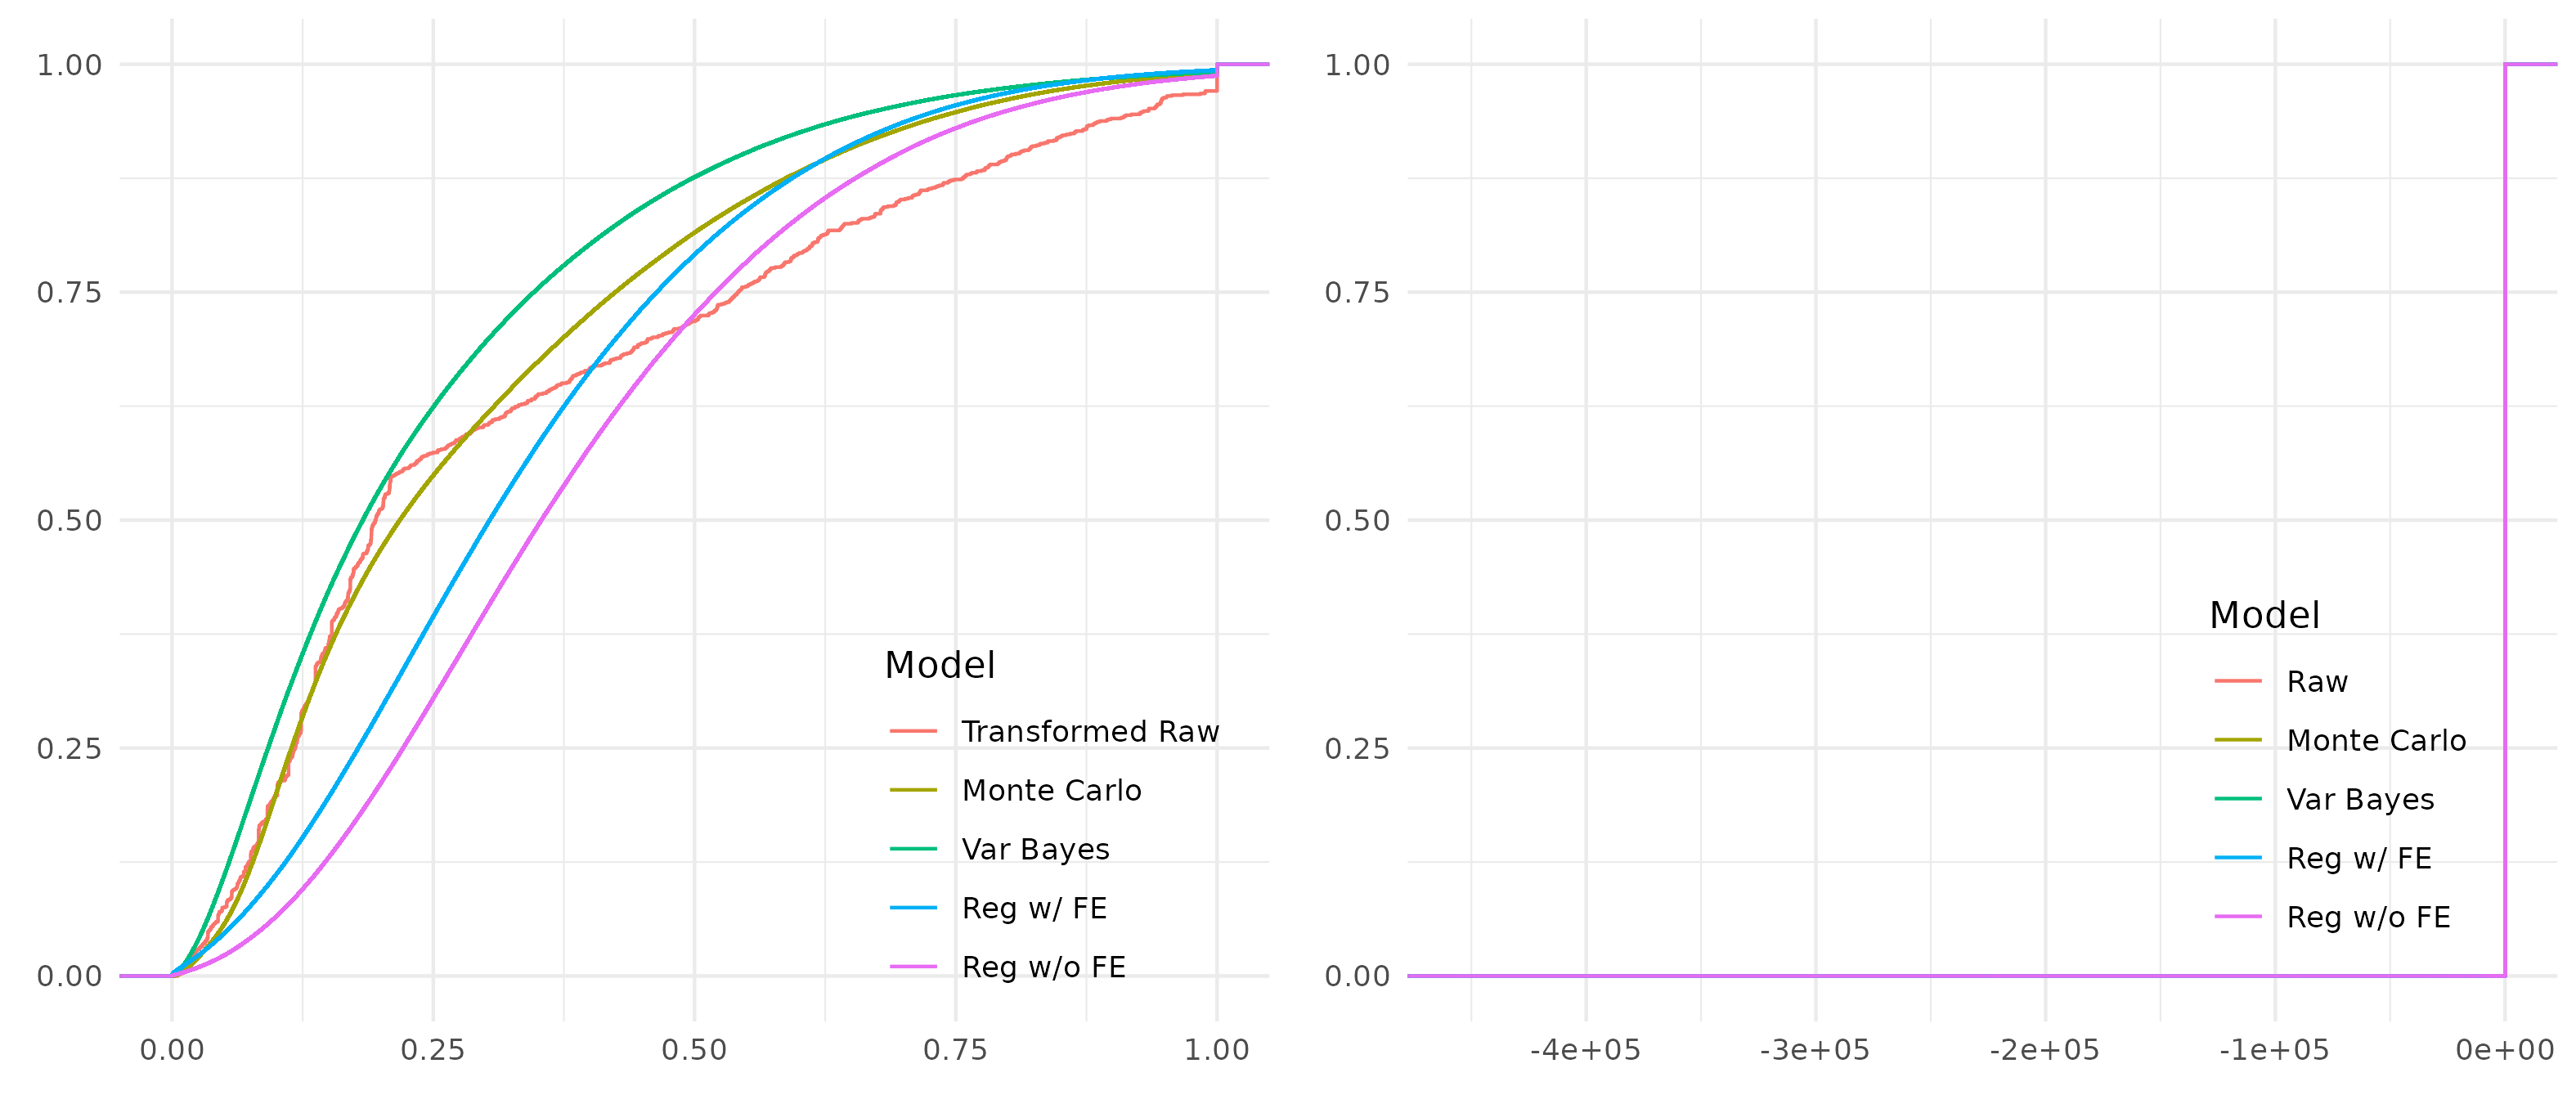
\includegraphics[width=\textwidth]{./plots/delaware_marginal_dover_afb.png}
%     \end{subfigure}
%     \\\vspace{1cm}~\\
%     \begin{subfigure}{0.8\textwidth}
%         \caption{Philadelphia International Airport\label{plot:marginal_pia}}
%         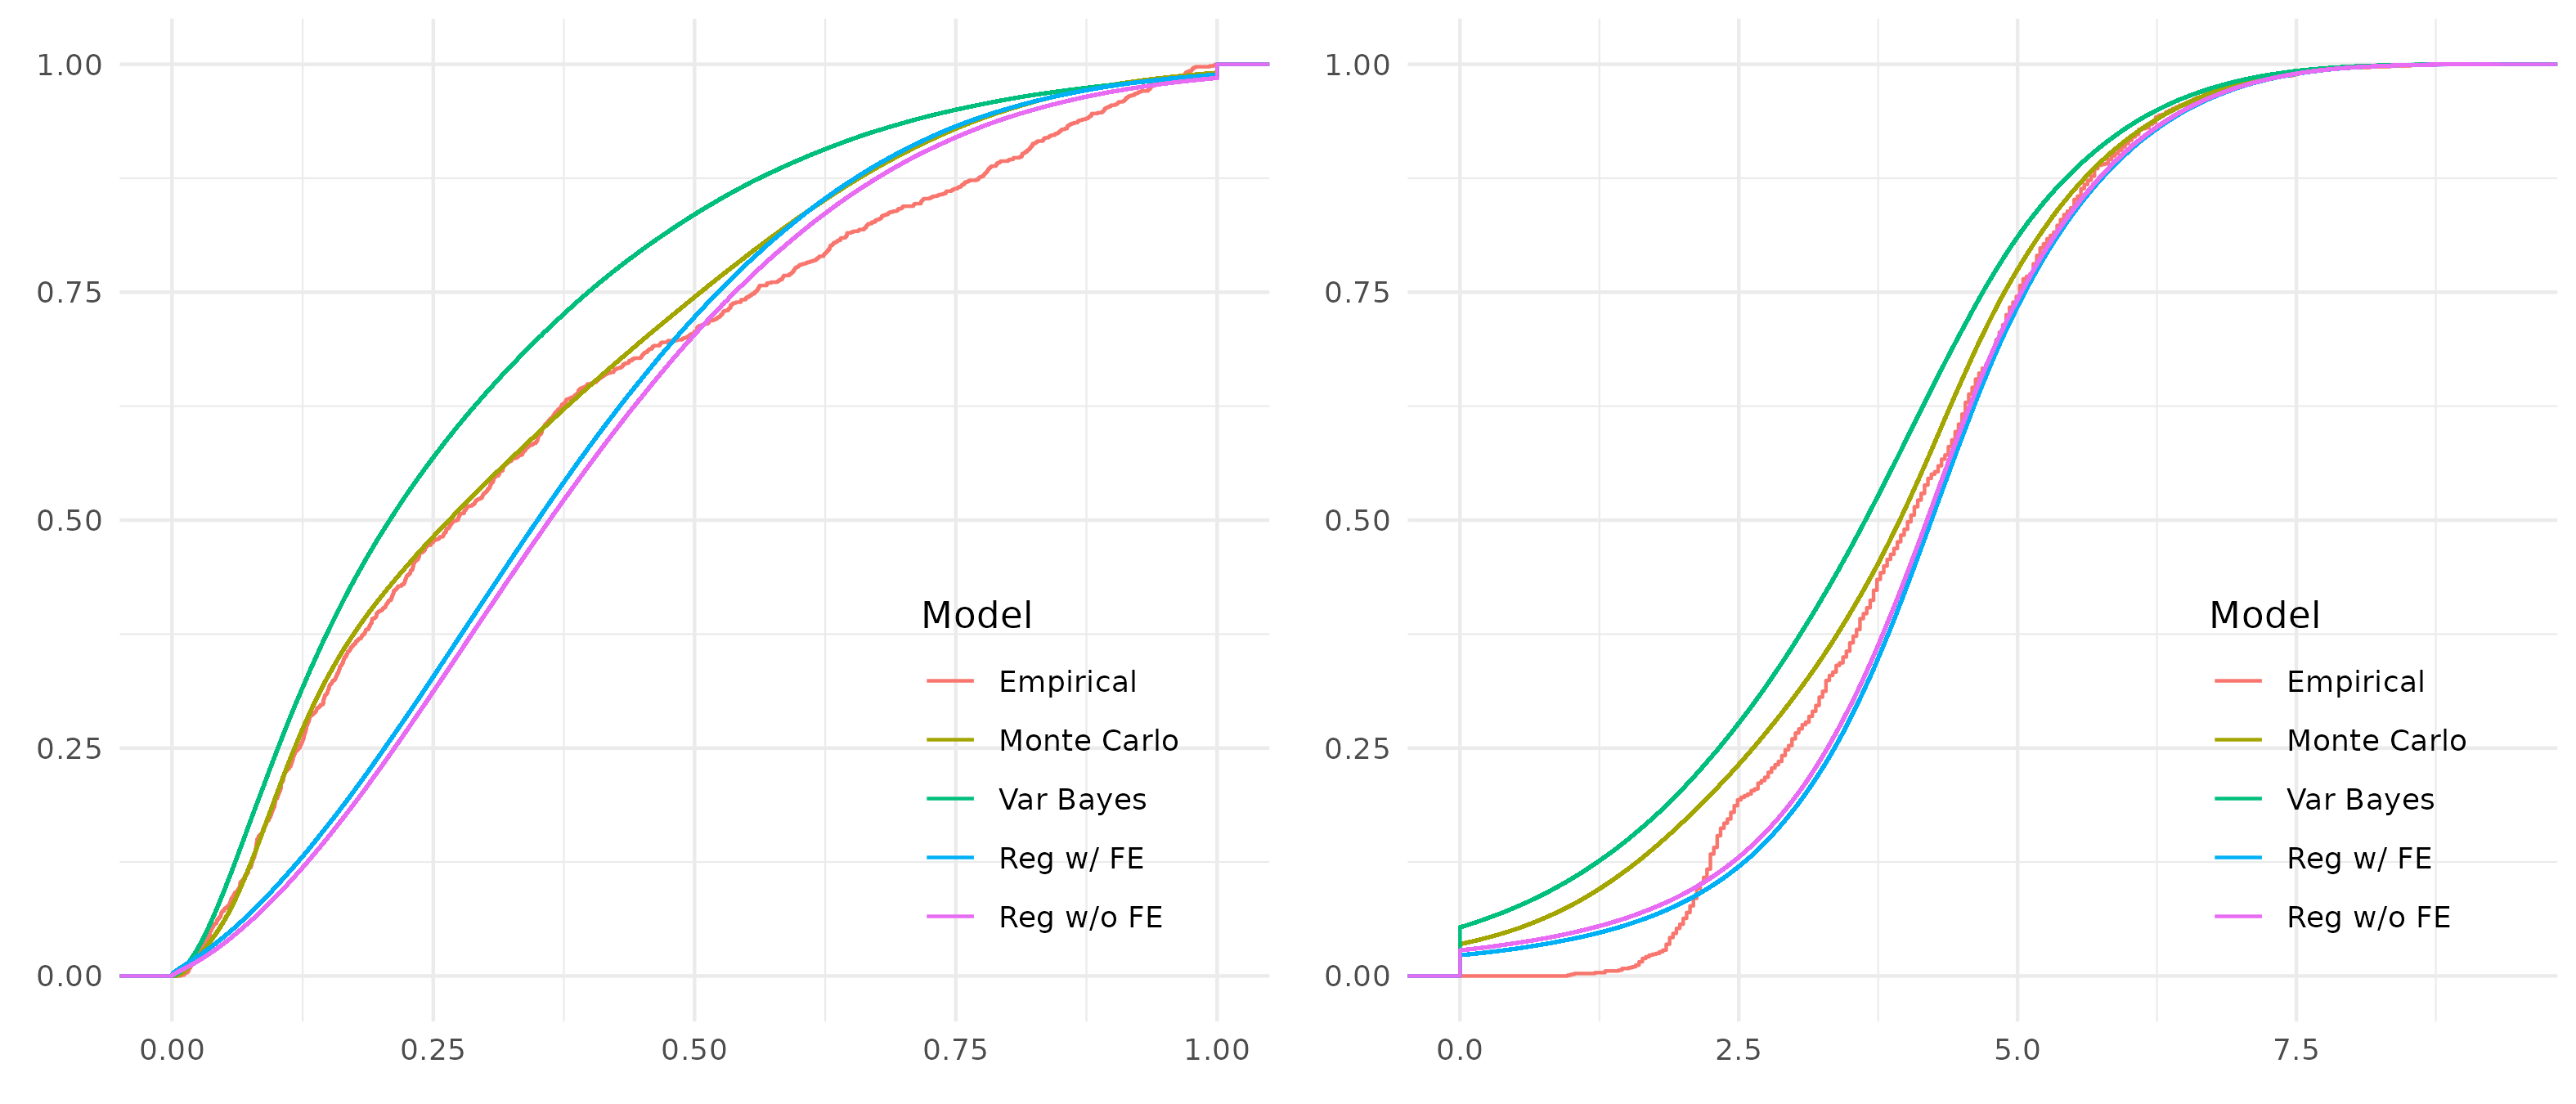
\includegraphics[width=\textwidth]{./plots/delaware_marginal_phil_ia.png}    
%     \end{subfigure}
%     \caption{Empirical, and posterior predictive cumulative distribution functions for marginal 
%     $v$, $V^*$ (Left) and $w$, $W^*$ (Right), at denoted locations, under various modeling
%     considerations.\makenote{remove legend name, compress into single faceted plot per location. 
%     make plot for packer terminal?}}
% \end{figure}

\begin{figure}[ht]
    \centering
    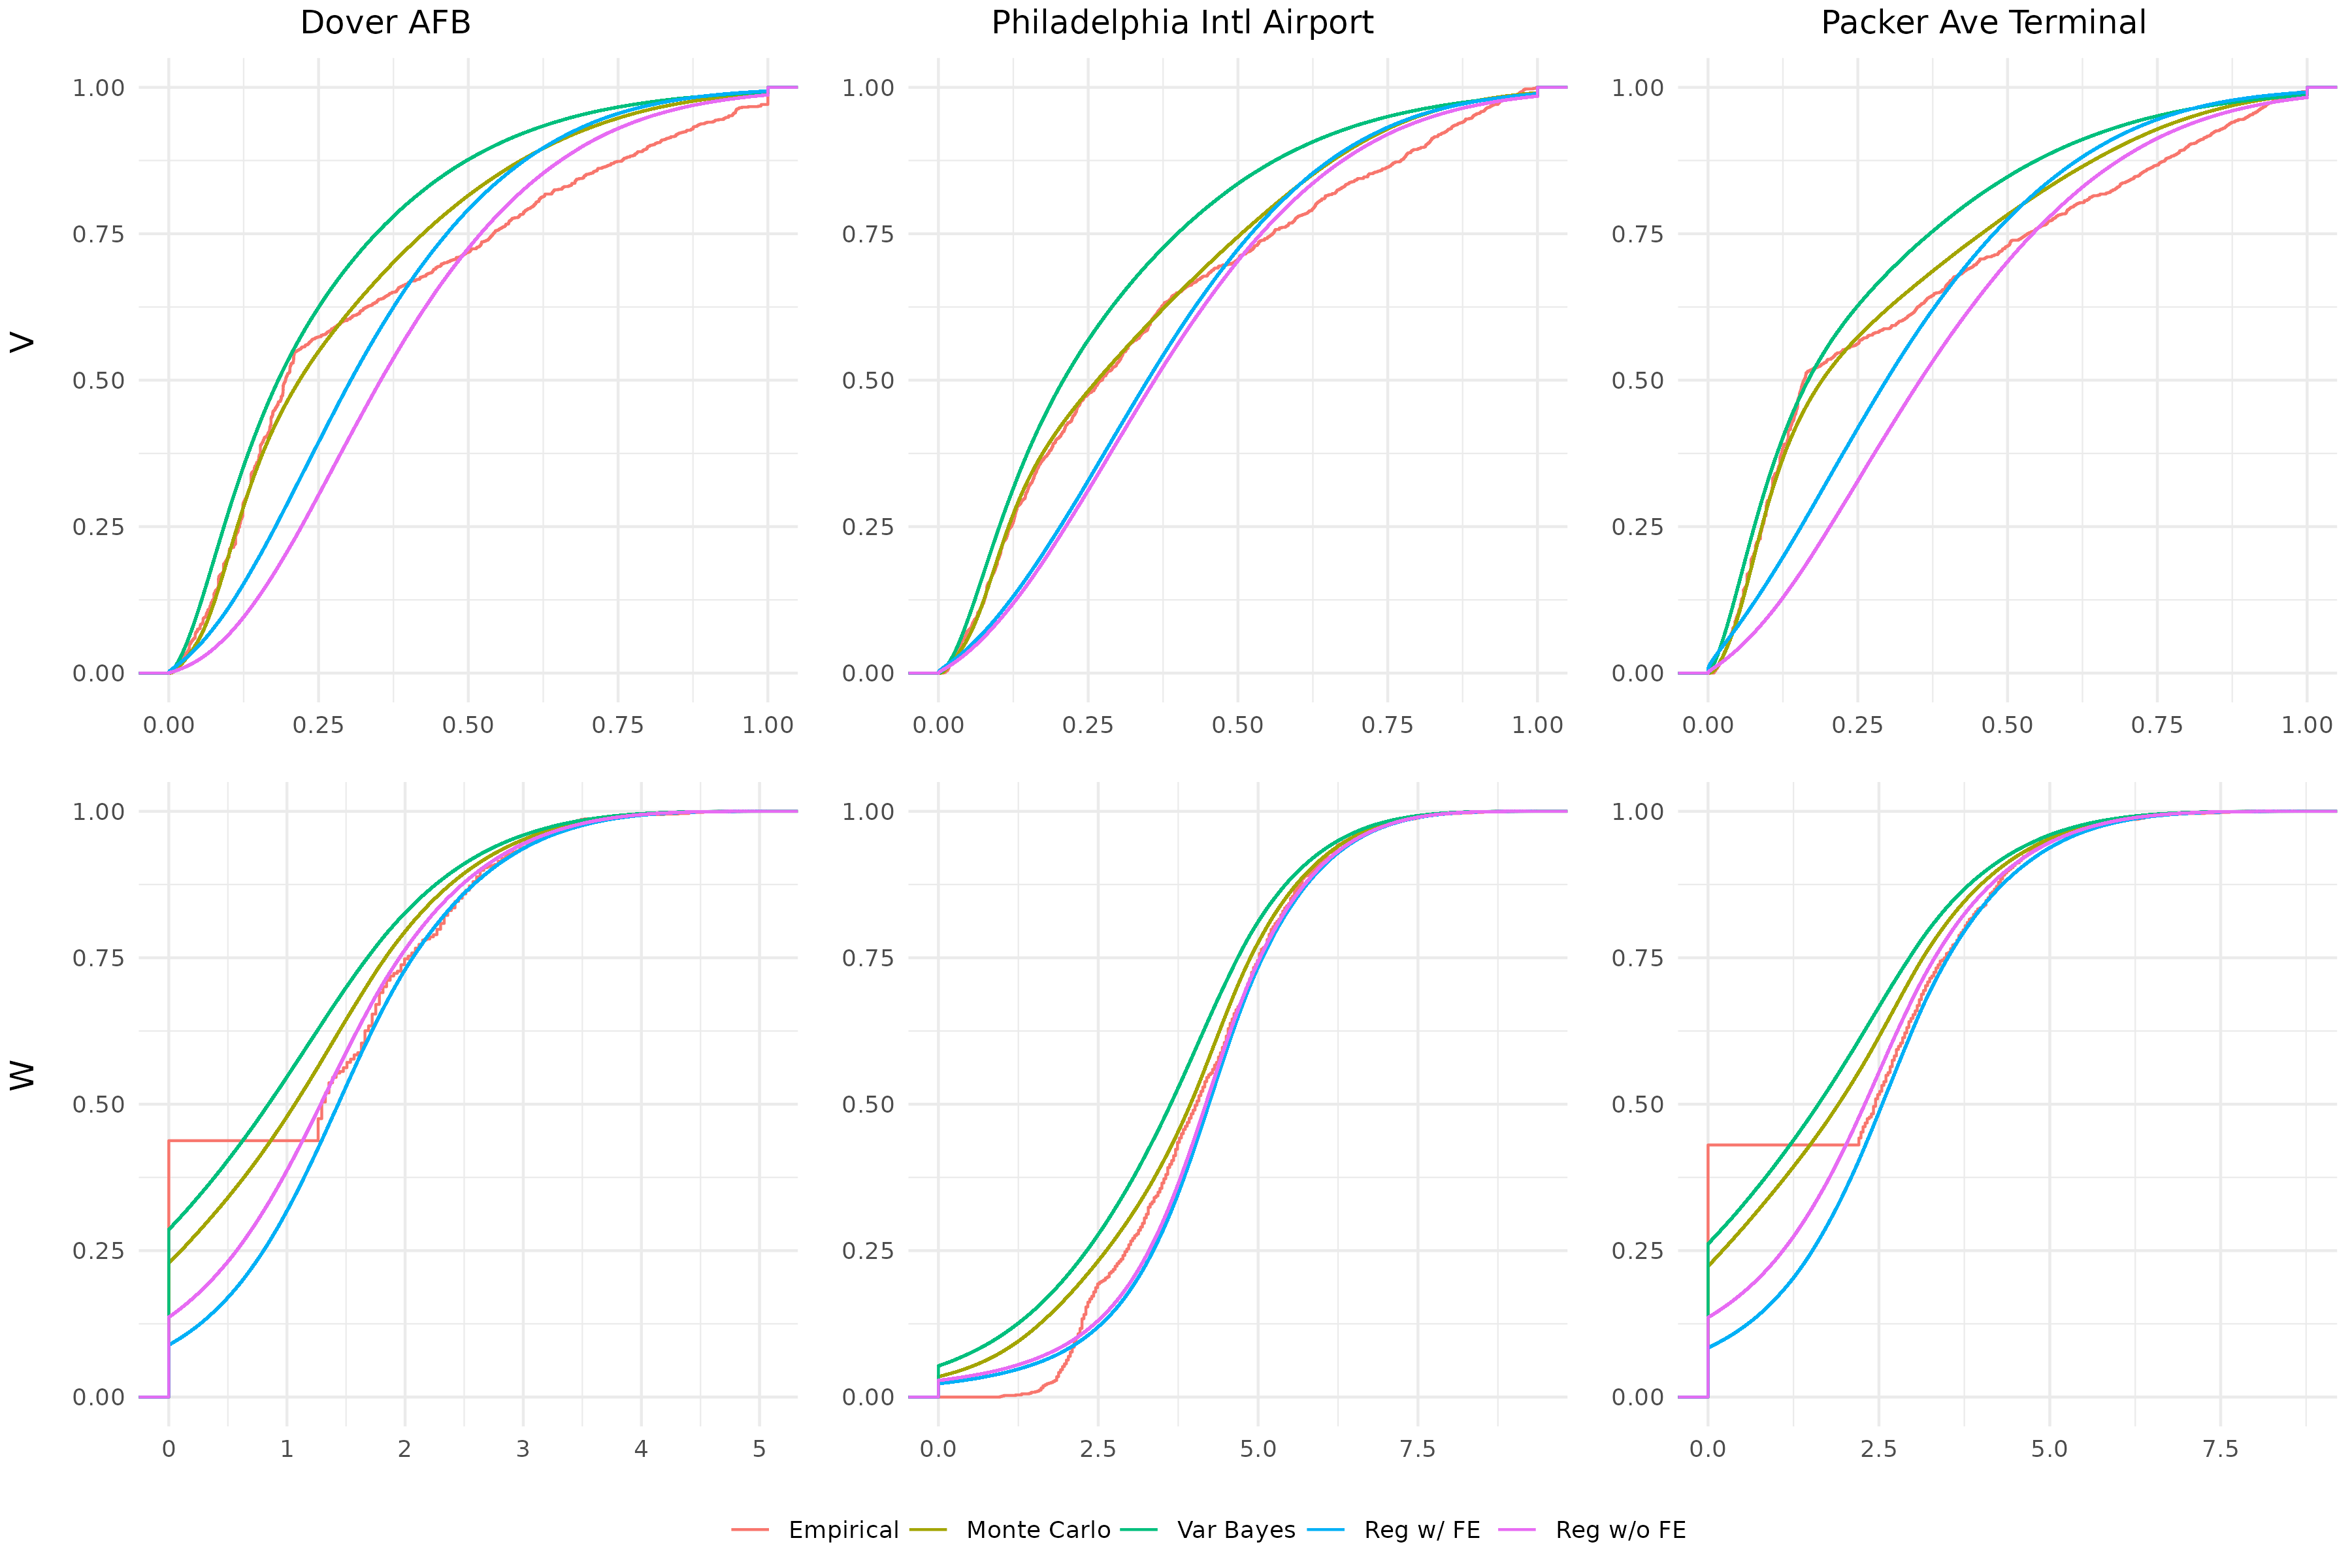
\includegraphics[width=0.95\linewidth]{./plots/delaware_marginal_cdfs.png}


In Figure~\ref{plot:marginal_doverafb}, we observe the marginal empirical and posterior-predictive
    CDF's for storm surge at Dover Air Force Base.  As previously mentioned, this location is adjacent
    to Delaware Bay, approximately 2 miles inland, with a direct line of sight out the mouth of the
    bay towards the open ocean.  Take note in particular, that the empirical CDF of $\bm{w}_s$ shows
    that storm surge does not reach Dover AFB in approximately \num{44} percent of storms, 
    post-thresholding.
In Figure~\ref{plot:marginal_pia}, we see the same marginal CDF's, for the Philadelphia International
    Airport.  Recall, this airport is situated along the banks of the Delaware River; storm surge
    has much further to travel to reach this point, and yet it experiences inundation much more 
    frequently, owing to the fact that its elevation is only 4 feet above sea level, 
    rather than the 9 feet for Dover AFB \makenote{[confirm]}.

\begin{table}[ht]
\centering
\caption{Cluster concentration for identified models and fitting 
        methods, on the \emph{Restricted} Slice: columns specify quantiles 
        detailing the proportion of data contained within the table cells 
        indicated number of clusters.\label{tab:cluster_concentration}} 
% latex table generated in R 4.4.1 by xtable 1.8-4 package
% Thu Oct 10 16:19:13 2024
\begin{tabular}{lrrr}
  \hline
Model & 0.9 & 0.99 & 0.999 \\ 
  \hline
Monte Carlo & 14 & 19 & 19 \\ 
  Var Bayes & 5 & 5 & 6 \\ 
  Reg w/o FE & 81 & 106 & 116 \\ 
  Reg w/ FE & 86 & 113 & 123 \\ 
   \hline
\end{tabular}

\end{table}

Looking at equivalent marginal plots for all locations, nearly all preserve the
    same ordering, from top-left to bottom-right: first the Variational Bayes fit of PYPG, then the 
    Monte Carlo fit of the same model, then the regression models---though the specific ordering of
    the regression models changes.  The marginal empirical CDFs tends to bounce\makenote{[rephrase]}
    between the MCMC model, and the regression models.  This means that the variational fit
    tends to consistently predict lower values than is appropriate. This permits us some insight 
    to comment what effect granularity, or the number of extant clusters, has in model fidelity.
    In Table~\ref{tab:cluster_concentration}, we see detail the number of clusters, or Pitman-Yor
    process mixture components, identified in the dataset under the specified model and fitting 
    method.  Observe the large difference between the MCMC fitting method and the VB fitting
    method. 
    \makenote{table of average $\text{E}[\alpha_s]$ under each model, as well as 
    $\text{E}\left[\frac{\alpha_s}{\lVert\bm{\alpha}\rVert_{\infty}}\right]$}



    \bruno{\bf Let me see if I understand what you are trying to say. The CDFs obtained from the models with a 
    regression component are the ones that are closer to the empirical CDFs, right? And the variational Bayes 
    are the ones that are the farther, right? Taking this as a measure of the
    ability of the model to replicate the observed data (what you call
    fidelity), this provides an indication of goodness of fit, right? Looking at
    the number of clusters that are estimated from each of the different
    approaches, it looks like the larger the number of clusters, the closer the estimated 
    CDF is to the empirical one. That makes sense, as the empirical CDFhas not clusters, 
    every data point is a cluster. Is this the story you want to tell? Can you try doing
    that in a clearer way?}

\subsection{Conditional Survival Curves}
From Equation~\ref{eqn:condsurv}, we can obtain the conditional probability of
    exceeding a specified threshold for some set of components, given that other dimensions exceed their specified 
    threshold. Using the \emph{Critical} slice with a model fitted via MCMC, we use this equation to establish 
    conditional survival curves for three locations: Dover Air Force Base, Philadelphia International Airport, 
    as well as the Packer Avenue Marine Terminal, a major shipping hub.  Packer Avenue Terminal is only a few 
    miles up the Delaware River from PIA, so we may expect a strong association in extreme behavior between 
    those two locations. In keeping with our goal of a practical actionable metric, we 
    consider three scenarios where we observe extreme behavior further out in the bay than the positions of
    interest.  In the \emph{Lower Bay} scenario, we observe extreme behavior at sites on the south side of the 
    bay towards the entrance of the bay.  That is, a scenario in which sites 1,2, and 7 (Beebe Hospital, 
    Henlopen Memorial Park, and Smyrna Airport respectively) experienced storm surge at or above their
    respective 90th percentiles.  In the \emph{Upper Bay} scenario, we observe extreme behavior at sites 6,
    and 8 (Bay Island Fish and Wildlife Refuge, and Salem Airfield respectively), sites situated along the
    northern edge of Delaware Bay.  In the \emph{Mouth} scenario, we observe extreme behavior at all sites near
    the mouth of the bay.  This includes sites 1, 2, 3, and 4 (Beebe Hospital, Henlopen Memorial Park, 
    Paramount Airport, and the Cape Regional Medical Center). 

\begin{figure}[htb]
    \begin{subfigure}[t]{0.31\textwidth}
        \centering
        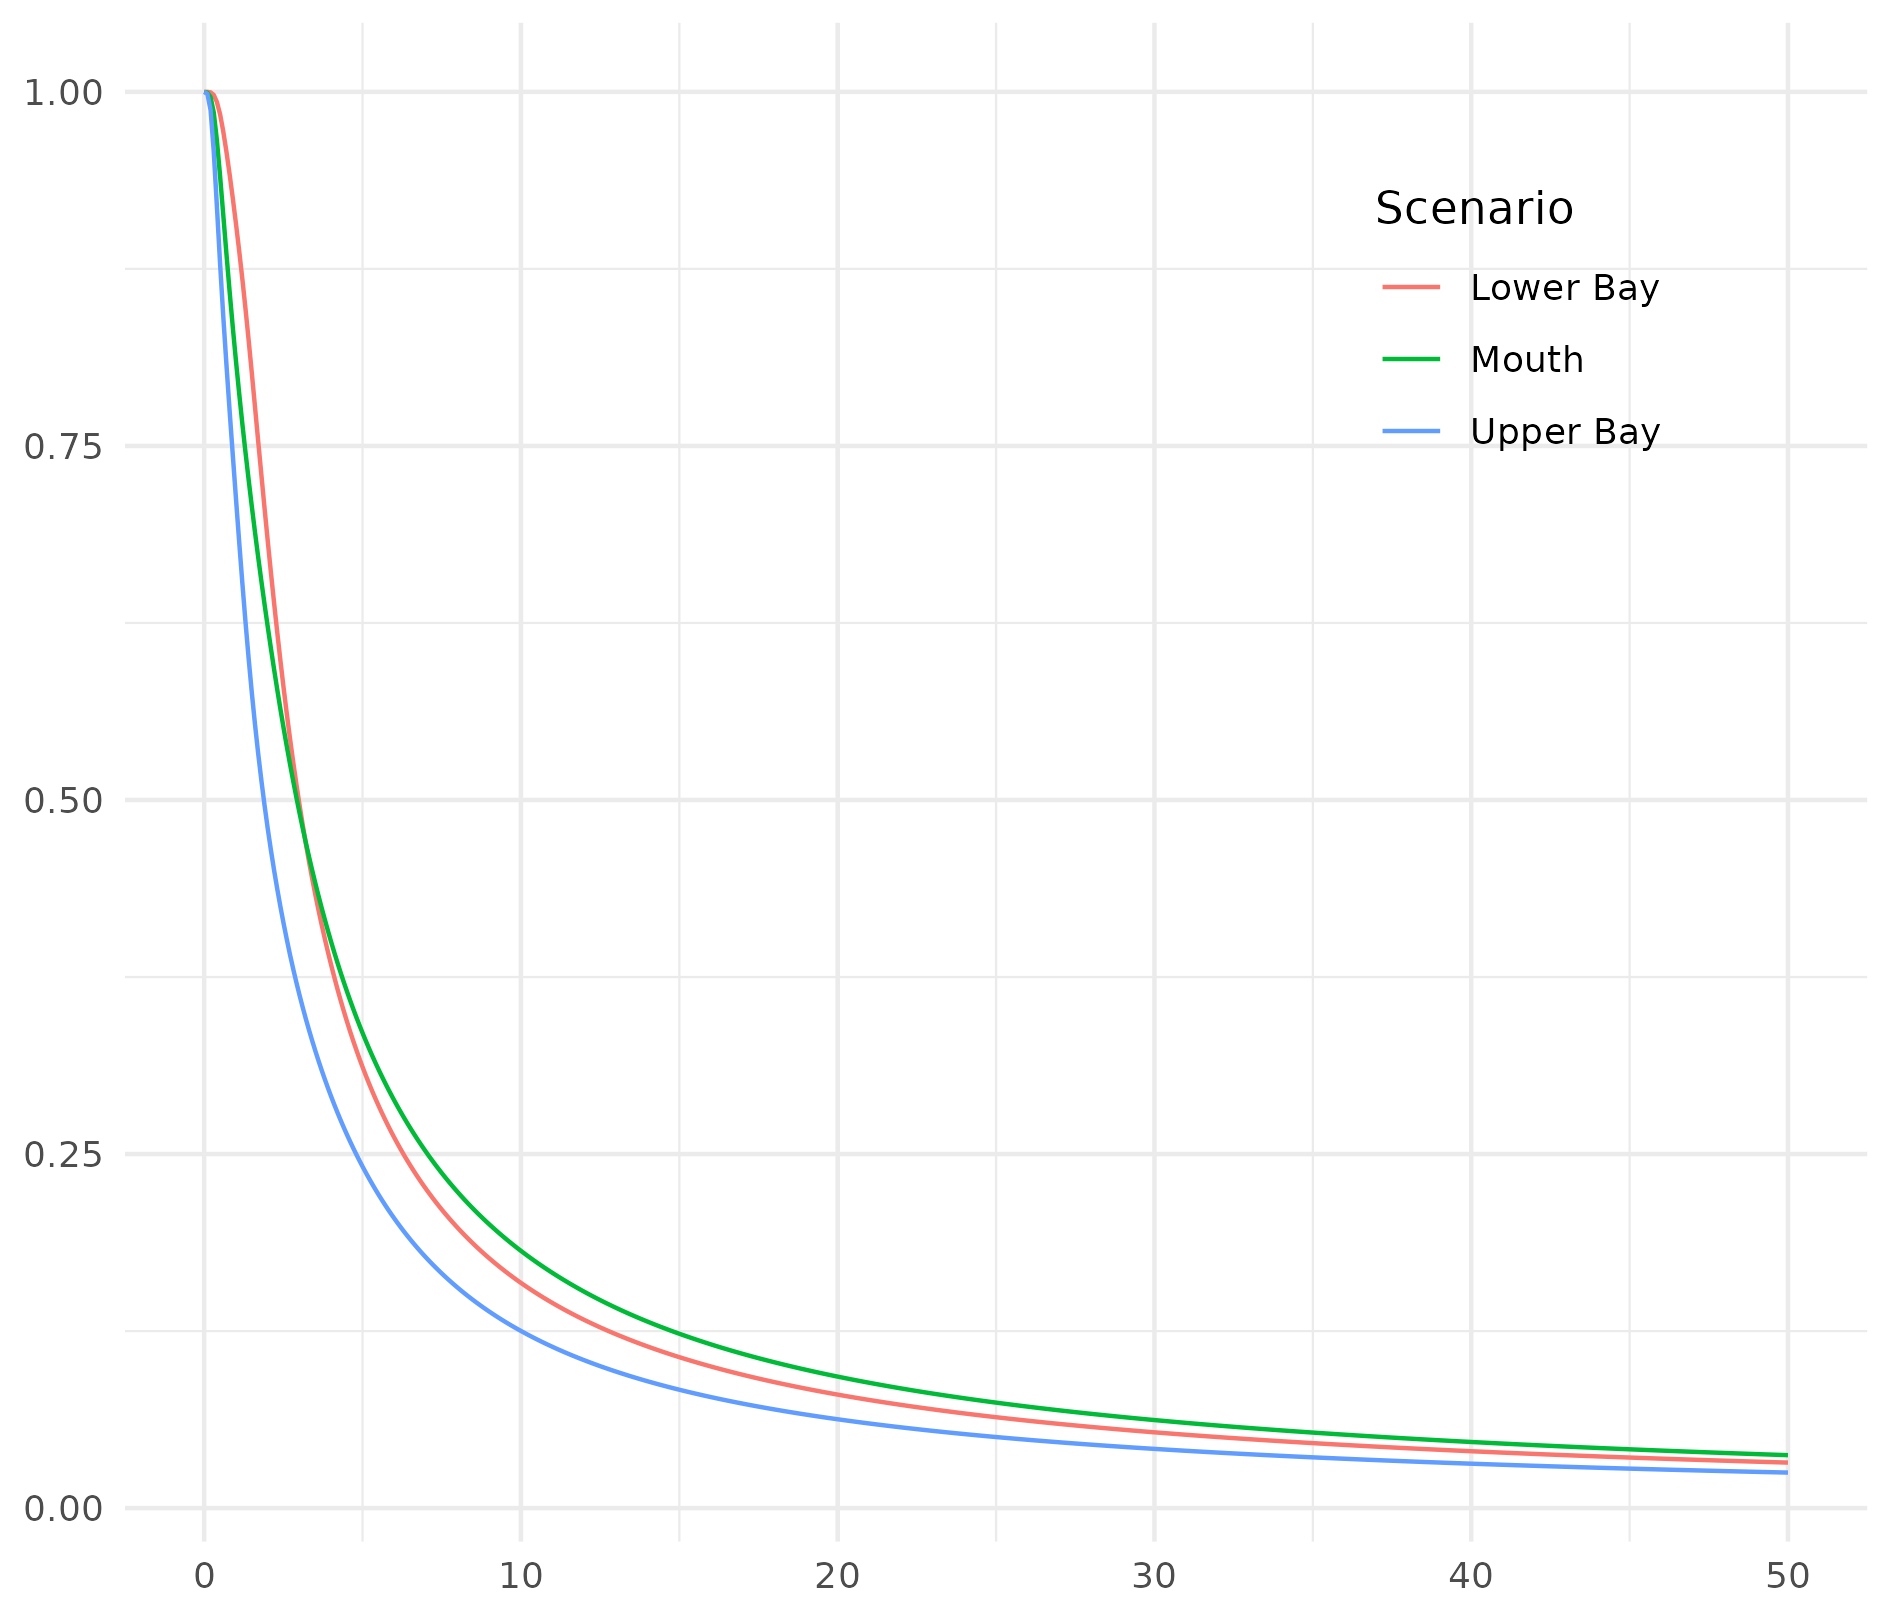
\includegraphics[width=0.99\linewidth]{./plots/condsurv/doverafb}
        \caption{Dover Air Force Base\label{fig:condsurv1d:doverafb}}
    \end{subfigure}%
    ~ 
    \begin{subfigure}[t]{0.31\textwidth}
        \centering
        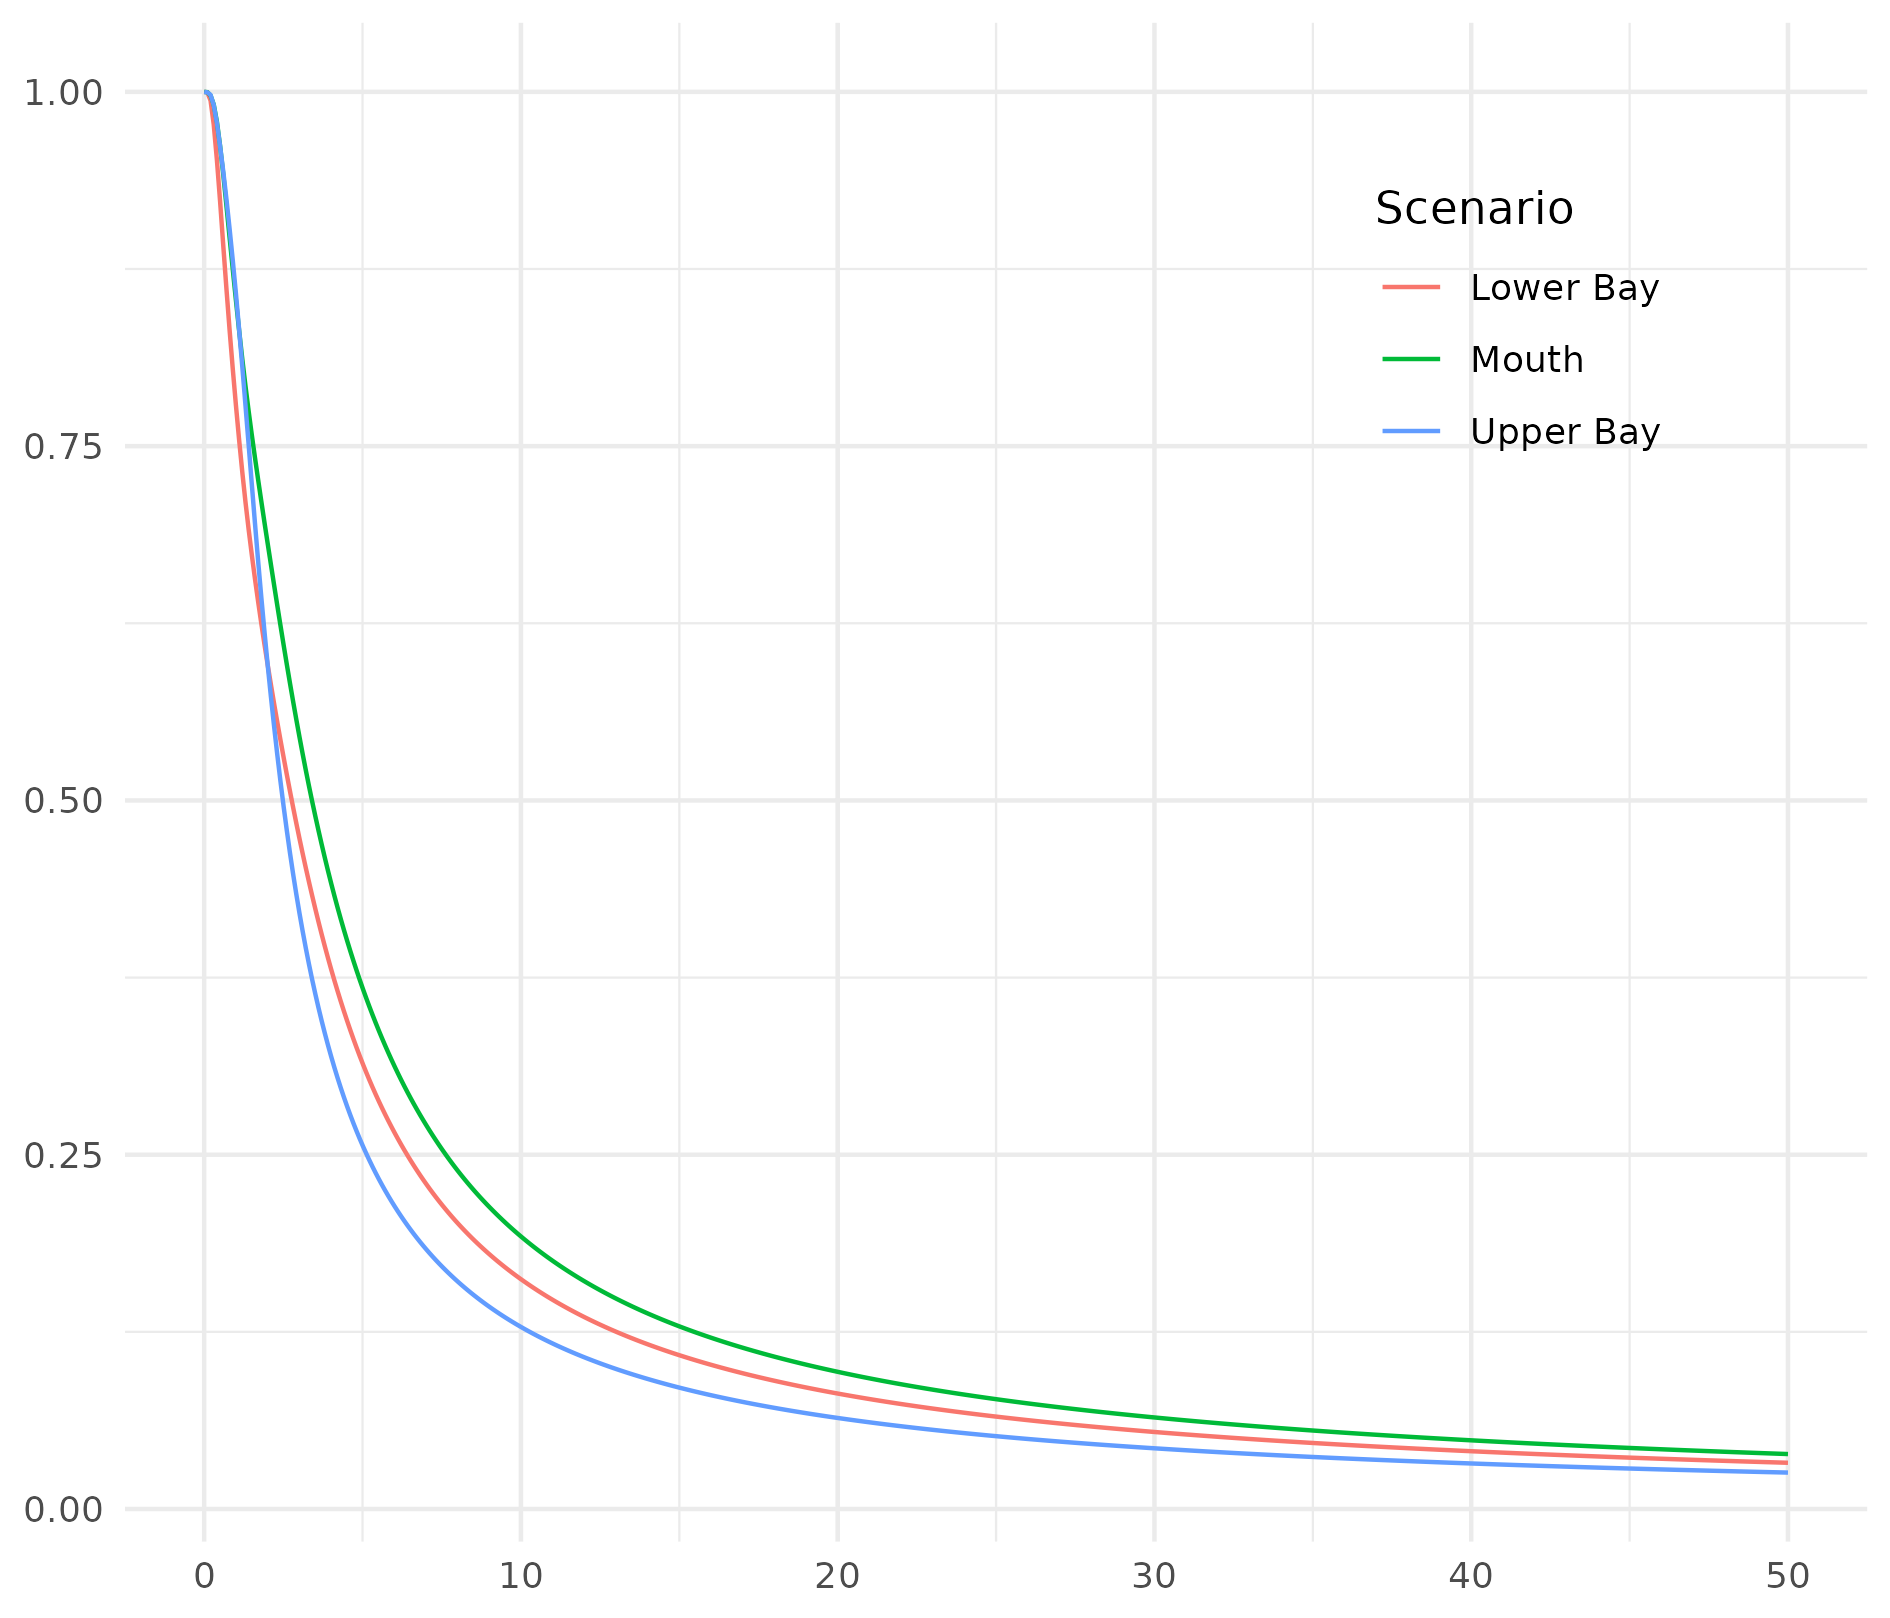
\includegraphics[width=0.99\linewidth]{./plots/condsurv/pia}
        \caption{Philadelphia International Airport\label{fig:condsurv1d:pia}}
    \end{subfigure}%
    ~
    \begin{subfigure}[t]{0.31\textwidth}
        \centering
        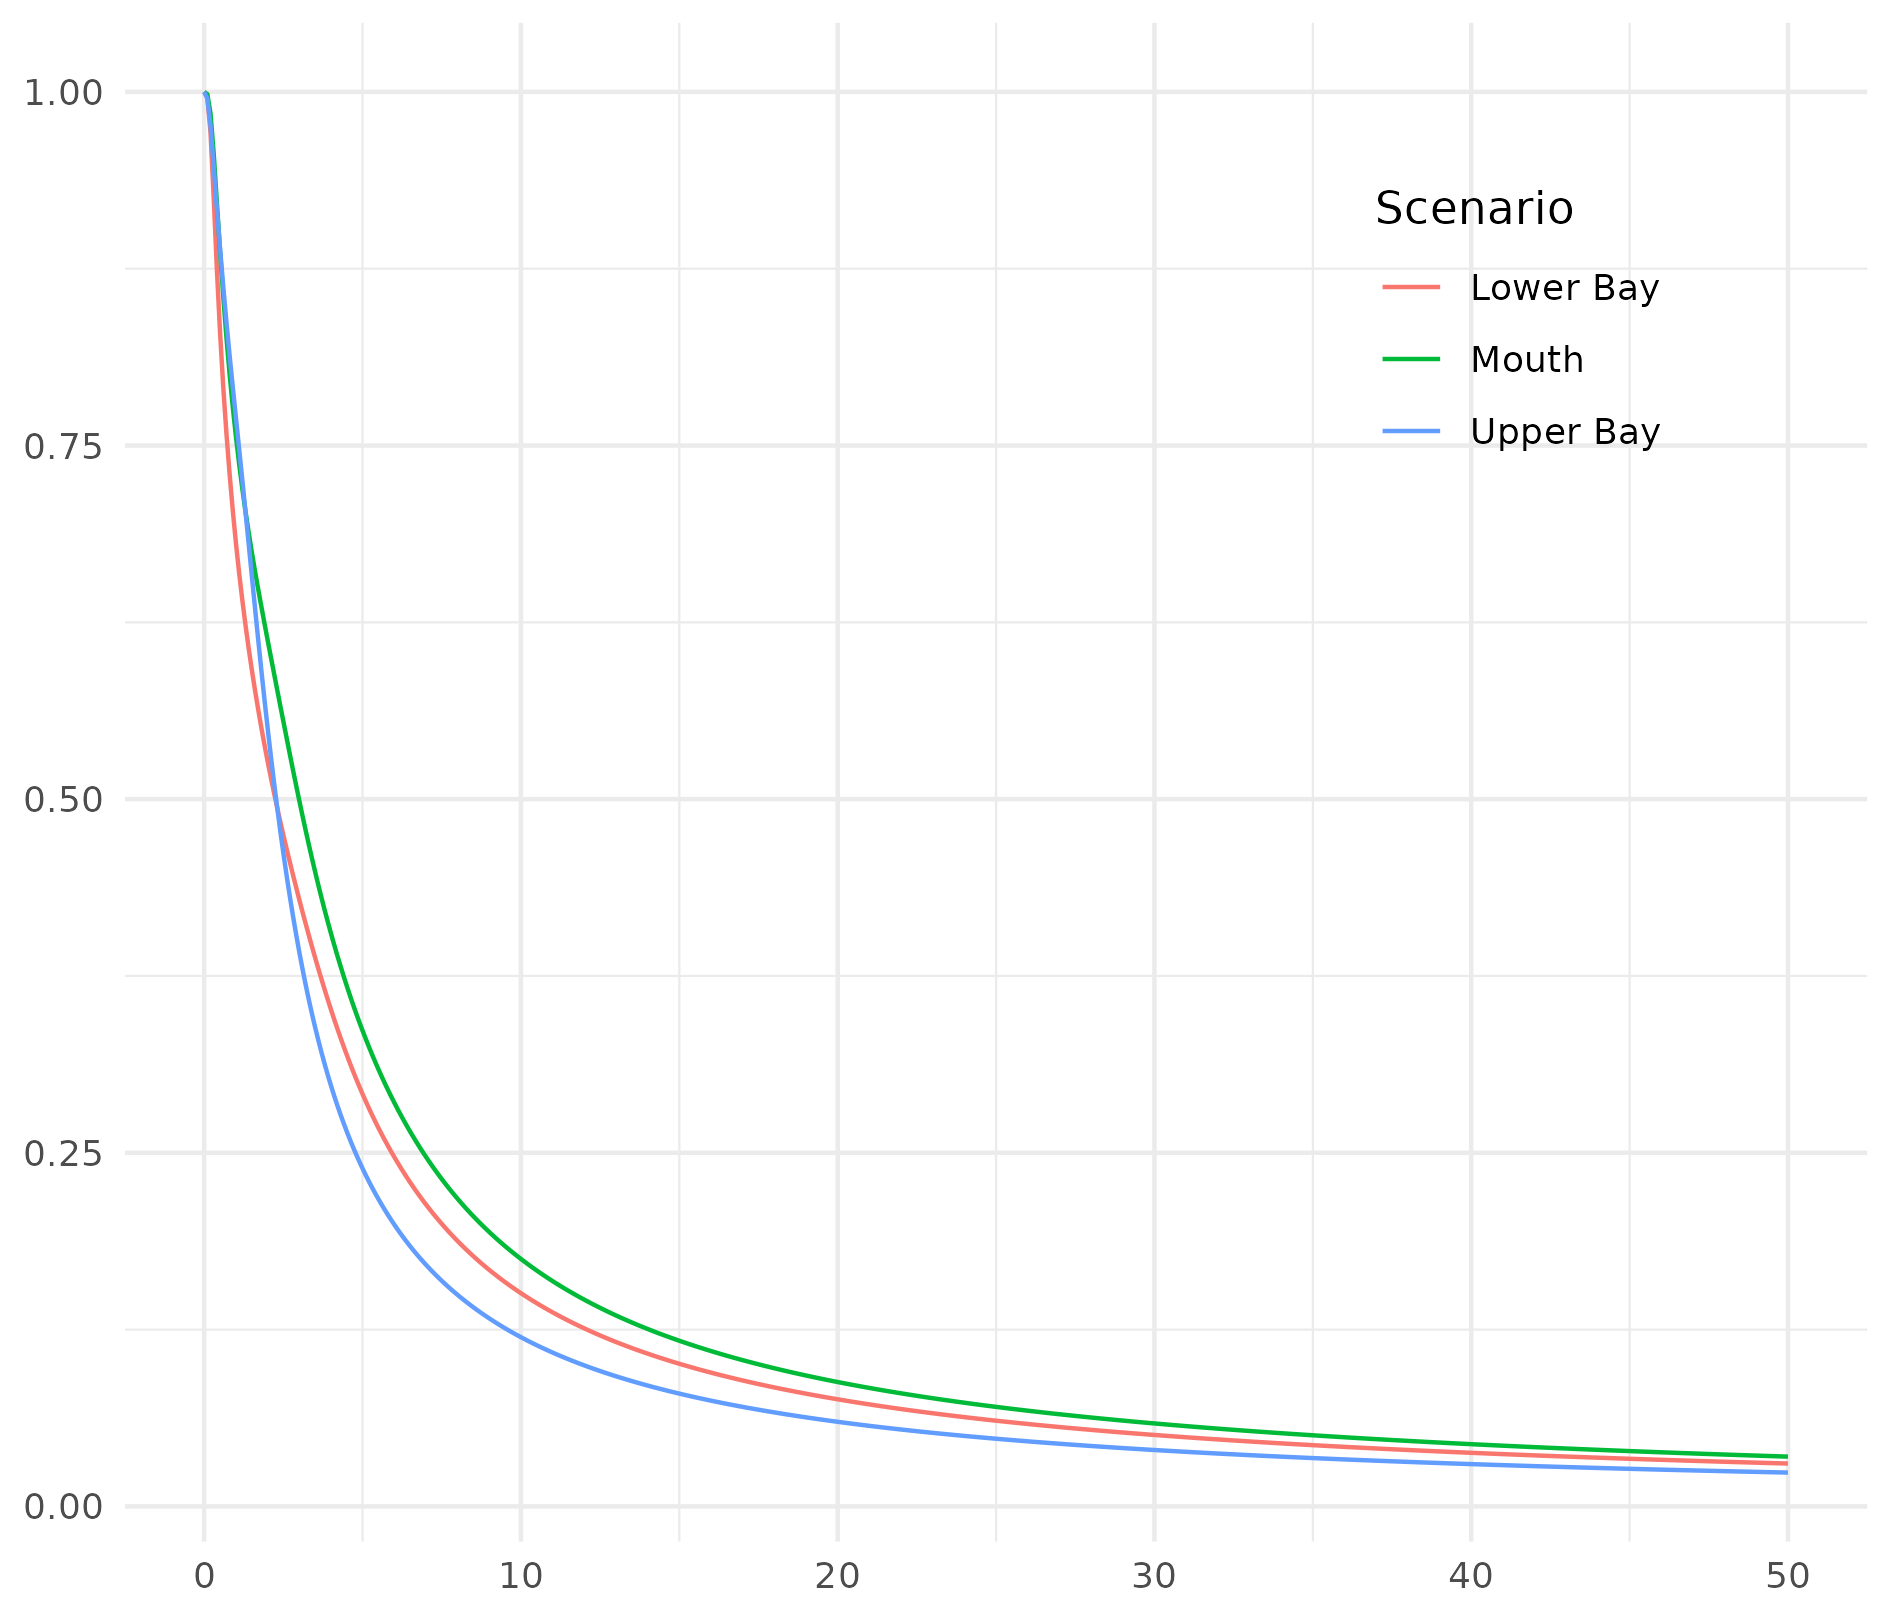
\includegraphics[width=\linewidth]{./plots/condsurv/packerave}
        \caption{Packer Avenue Marine Terminal\label{fig:condsurv1d:packerave}}
    \end{subfigure}
    \caption{Conditional survival curves for the labelled locations, under three scenarios of the observed \label{fig:condsurv1d}}
\end{figure}

Figure~\ref{fig:condsurv1d} shows the one-dimensional survival curves for these three locations, under 
    these three scenarios.  Note, the survival curve indicates $P(Z_s > z_s)$ given the stated scenario.
    Additionally, a $\bm{z}$ score greater than 1 indicates storm surge above the 90th percentile.
    Perhaps unsurprisingly in interpreting these results, as Dover AFB is on the south side of the bay, 
    we see the survival curve for the Upper Bay scenario dip below that of both Lower Bay and Mouth scenarios.  
    What is interesting, however, is that that ordering is not uniform; we see the ordering change to that
    behavior around $z = 4$.  The Mouth scenario indicates a storm that has inundated both the lower and
    upper portions of the Delaware Bay entrance, indicating an extremely powerful storm that is well positioned
    to enter the Bay.  As such, it is no surprise that the survival curve associated with that scenario
    indicates the highest probability of extreme surge throughout the entire curve.  What is interesting is that
    we observe the same crossing behavior and the same ordering on all three curves, though their exact shape
    and the exact point at which that cross occurs differ.  It is apparent that relative to the other
    scenarios, extreme surge on the Upper Bay sites does not strongly indicate increased surge at the other 
    sites.  It may be the case that a hurricane optimally aligned towards inundating the North bank is 
    sub-optimally aligned towards inundating the rest of the bay.

\begin{figure}[htb]
    \centering
    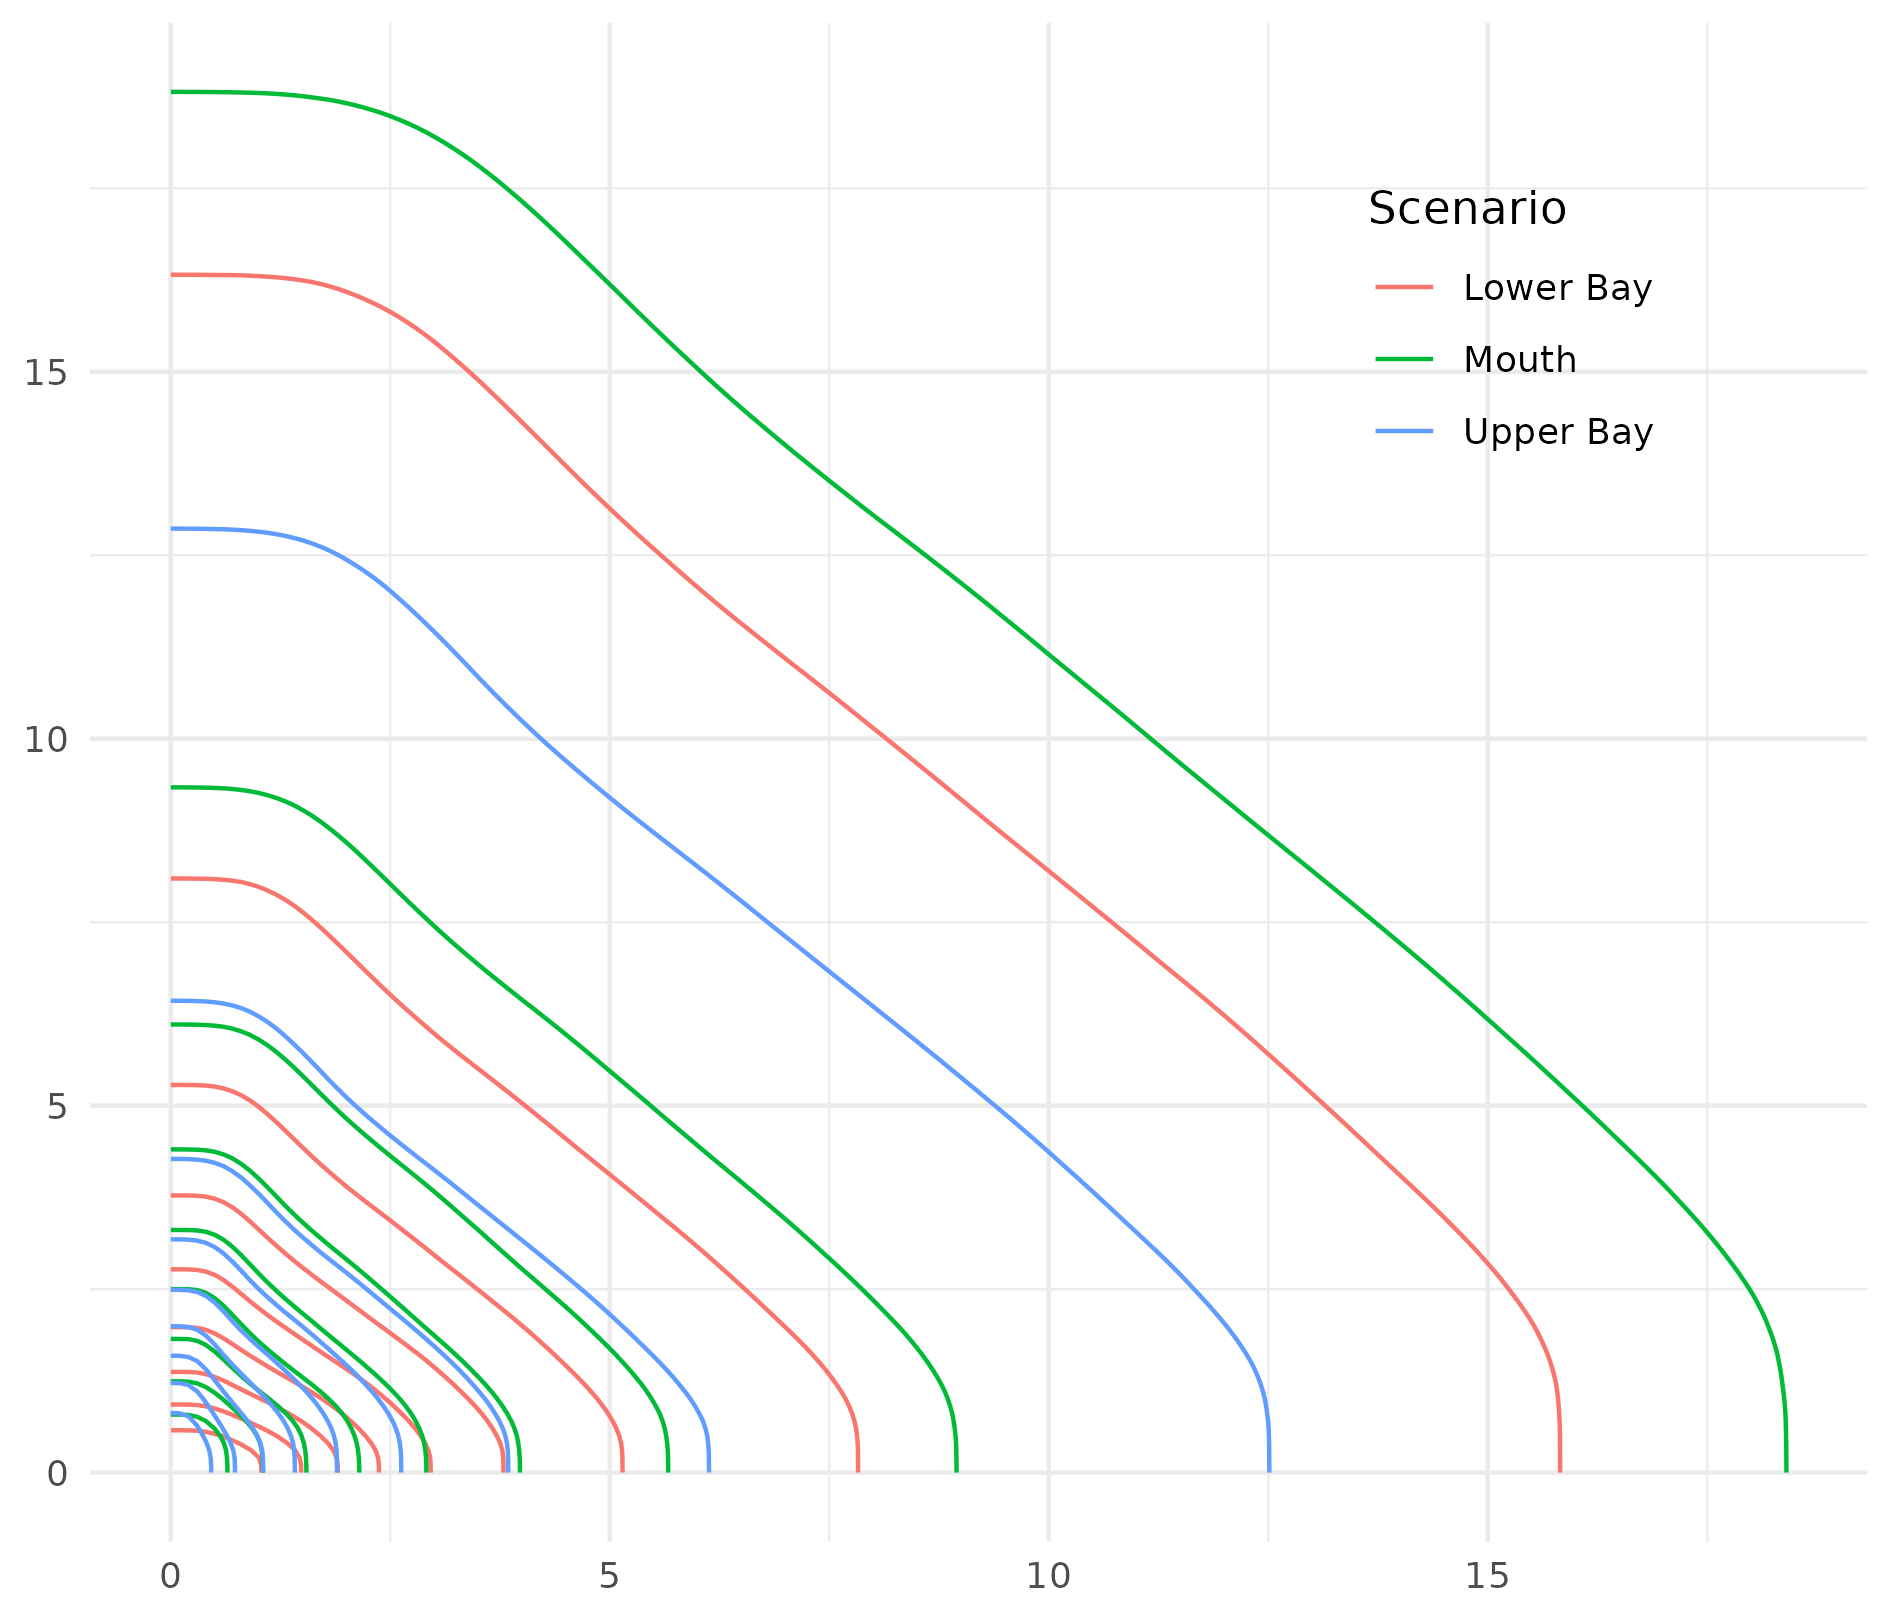
\includegraphics[width=0.3\linewidth]{./plots/condsurv/doverafb_pia}
    \caption{Conditional Survival Curve (Contour Plot) of flooding at Dover AFB (X) vs Philadelphia International 
        Airport (Y).\label{fig:condsurv2d:doverpia}
        \makenote{Add plot in real units}}
\end{figure}

\begin{figure}[htb]
    \centering
    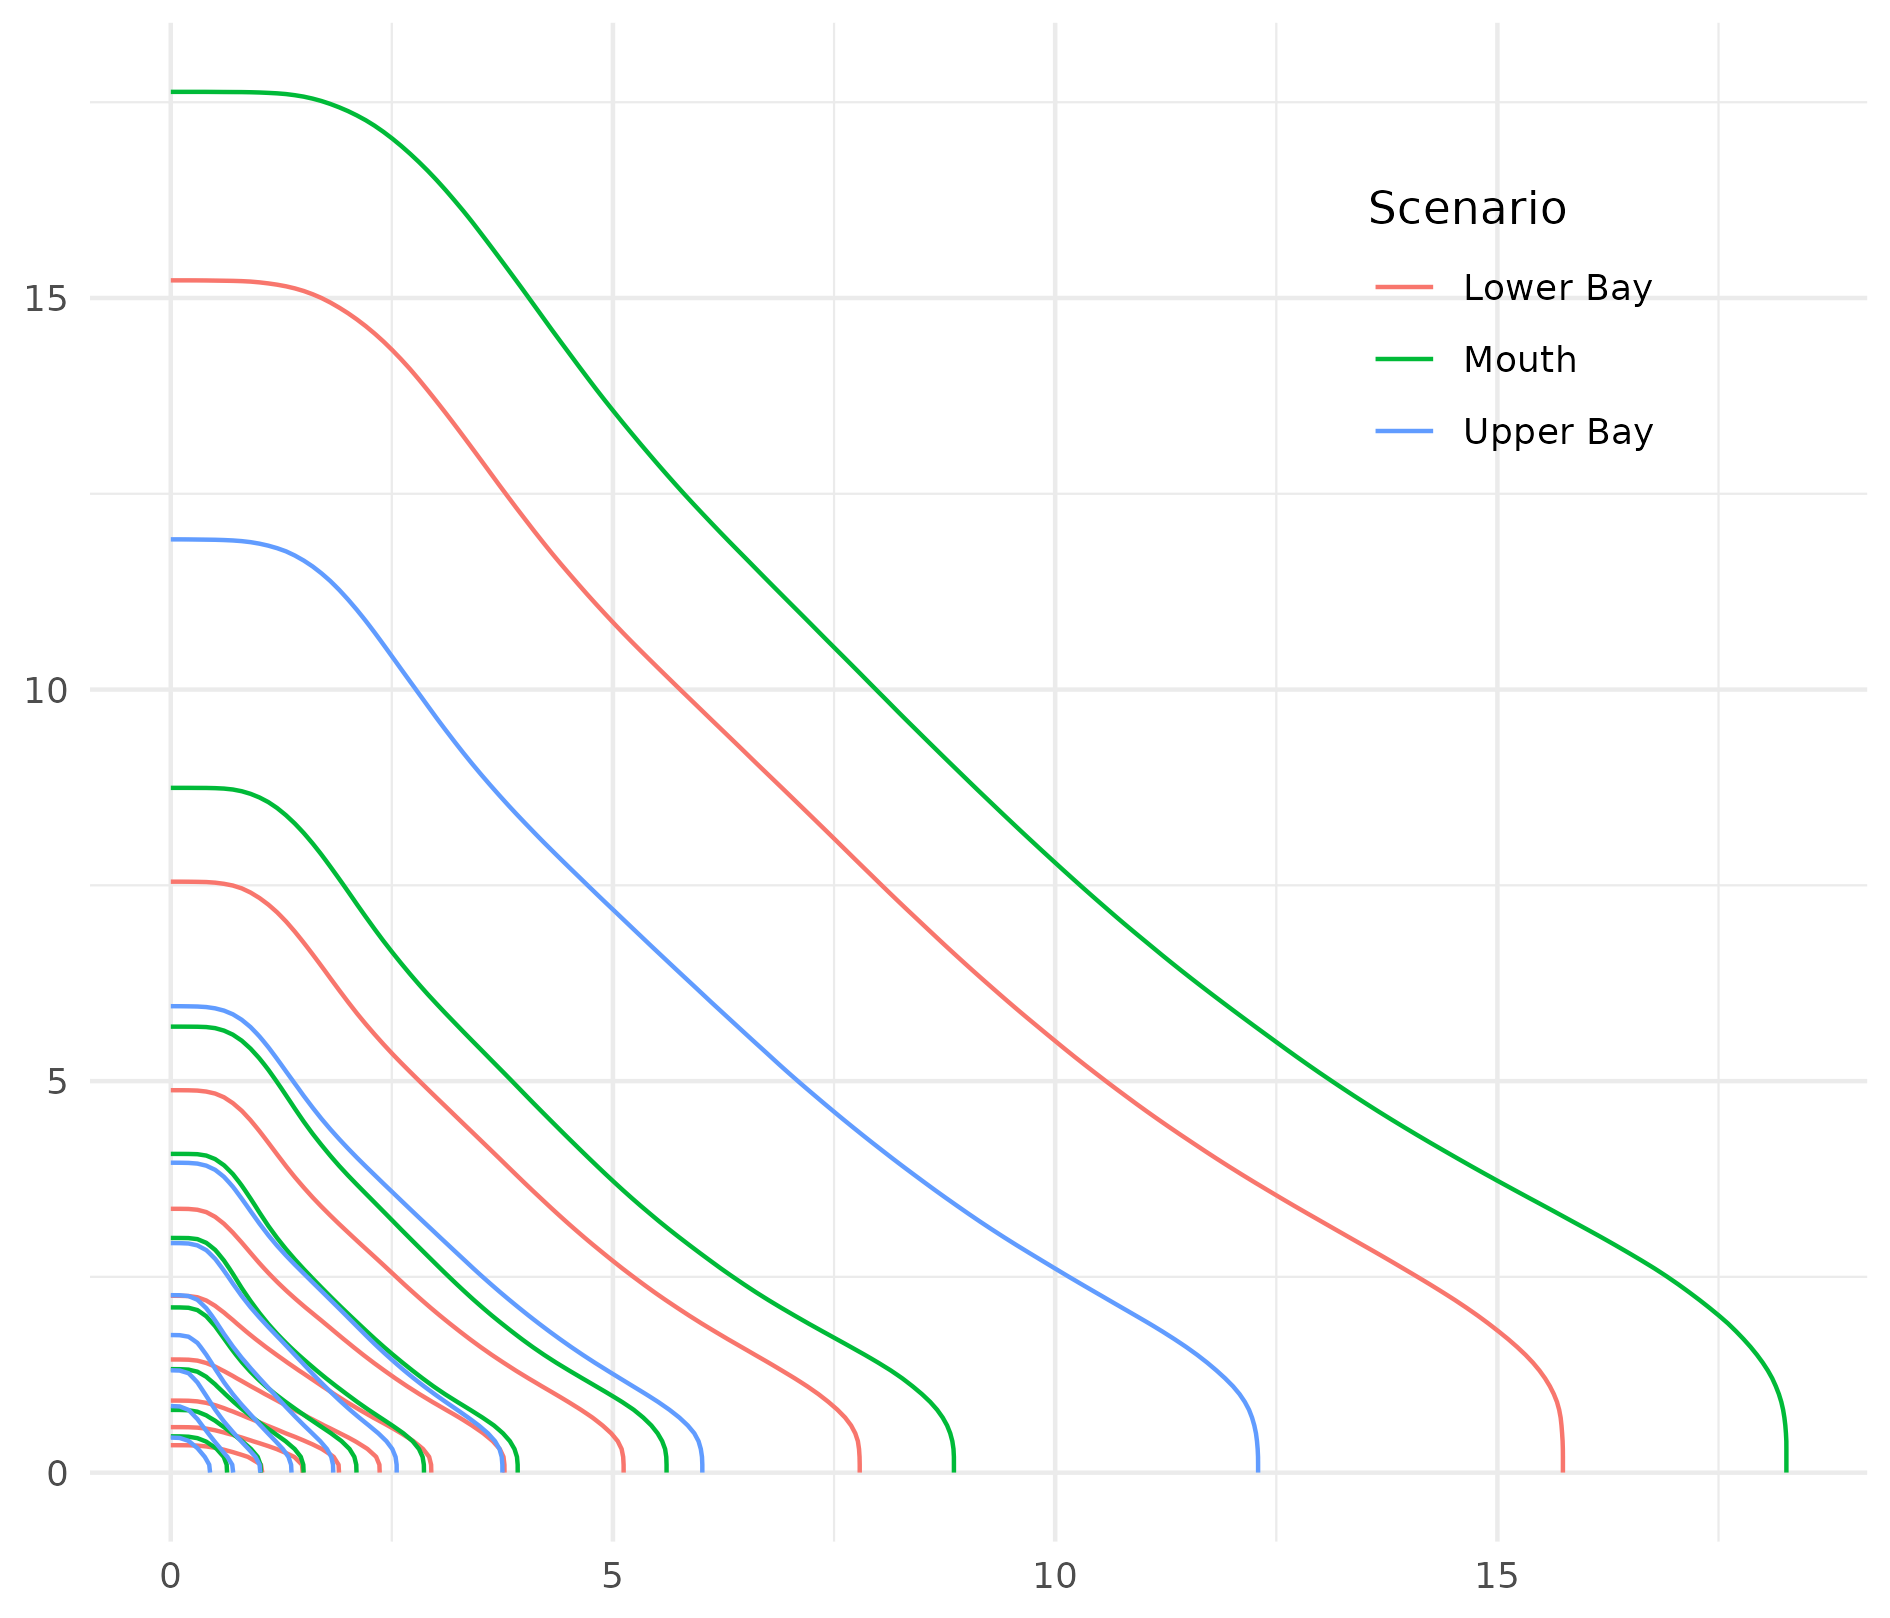
\includegraphics[width=0.3\linewidth]{./plots/condsurv/doverafb_packer}
    \caption{Conditional Survival Curve (Contour Plot) of flooding at Dover AFB (X) vs Packer Avenue Terminal (Y).
        \label{fig:condsurv2d:doverpacker}
        \makenote{Add plot in real units}
        }
\end{figure}

Figure~\ref{fig:condsurv2d:doverpia} provides a contour plot of a two-dimensional survival surface, between
    flooding at Dover AFB and flooding at PIA, conditional on the listed scenarios.  Recalling that Dover AFB 
    is on the south edge of the bay, while PIA is far up the Delaware River, we may not expect to see a strong
    association between the two locations.  Indeed, on the contour plot we observe the survival surface is nearly 
    flat on the transition between Dover AFB and PIA. \makenote{This phrasing is terrible.}  This shape indicates
    an only moderate dependence between the locations, under these scenarios.  But we must call 
    attention to the ordering of the contours of the survival surface.  Here, the Lower Bay scenario crosses 
    even the Mouth scenario.  In contrast, in Figure~\ref{fig:condsurv2d:doverpacker}, we see that survival
    surface is actually concave, which indicates an extremely weak dependence between the two 
    locations.  This is understandable, as Packer Avenue Terminal is around 4 miles upstream of PIA,
    even further away from Dover AFB.    
    
\begin{figure}[htb]
    \centering
    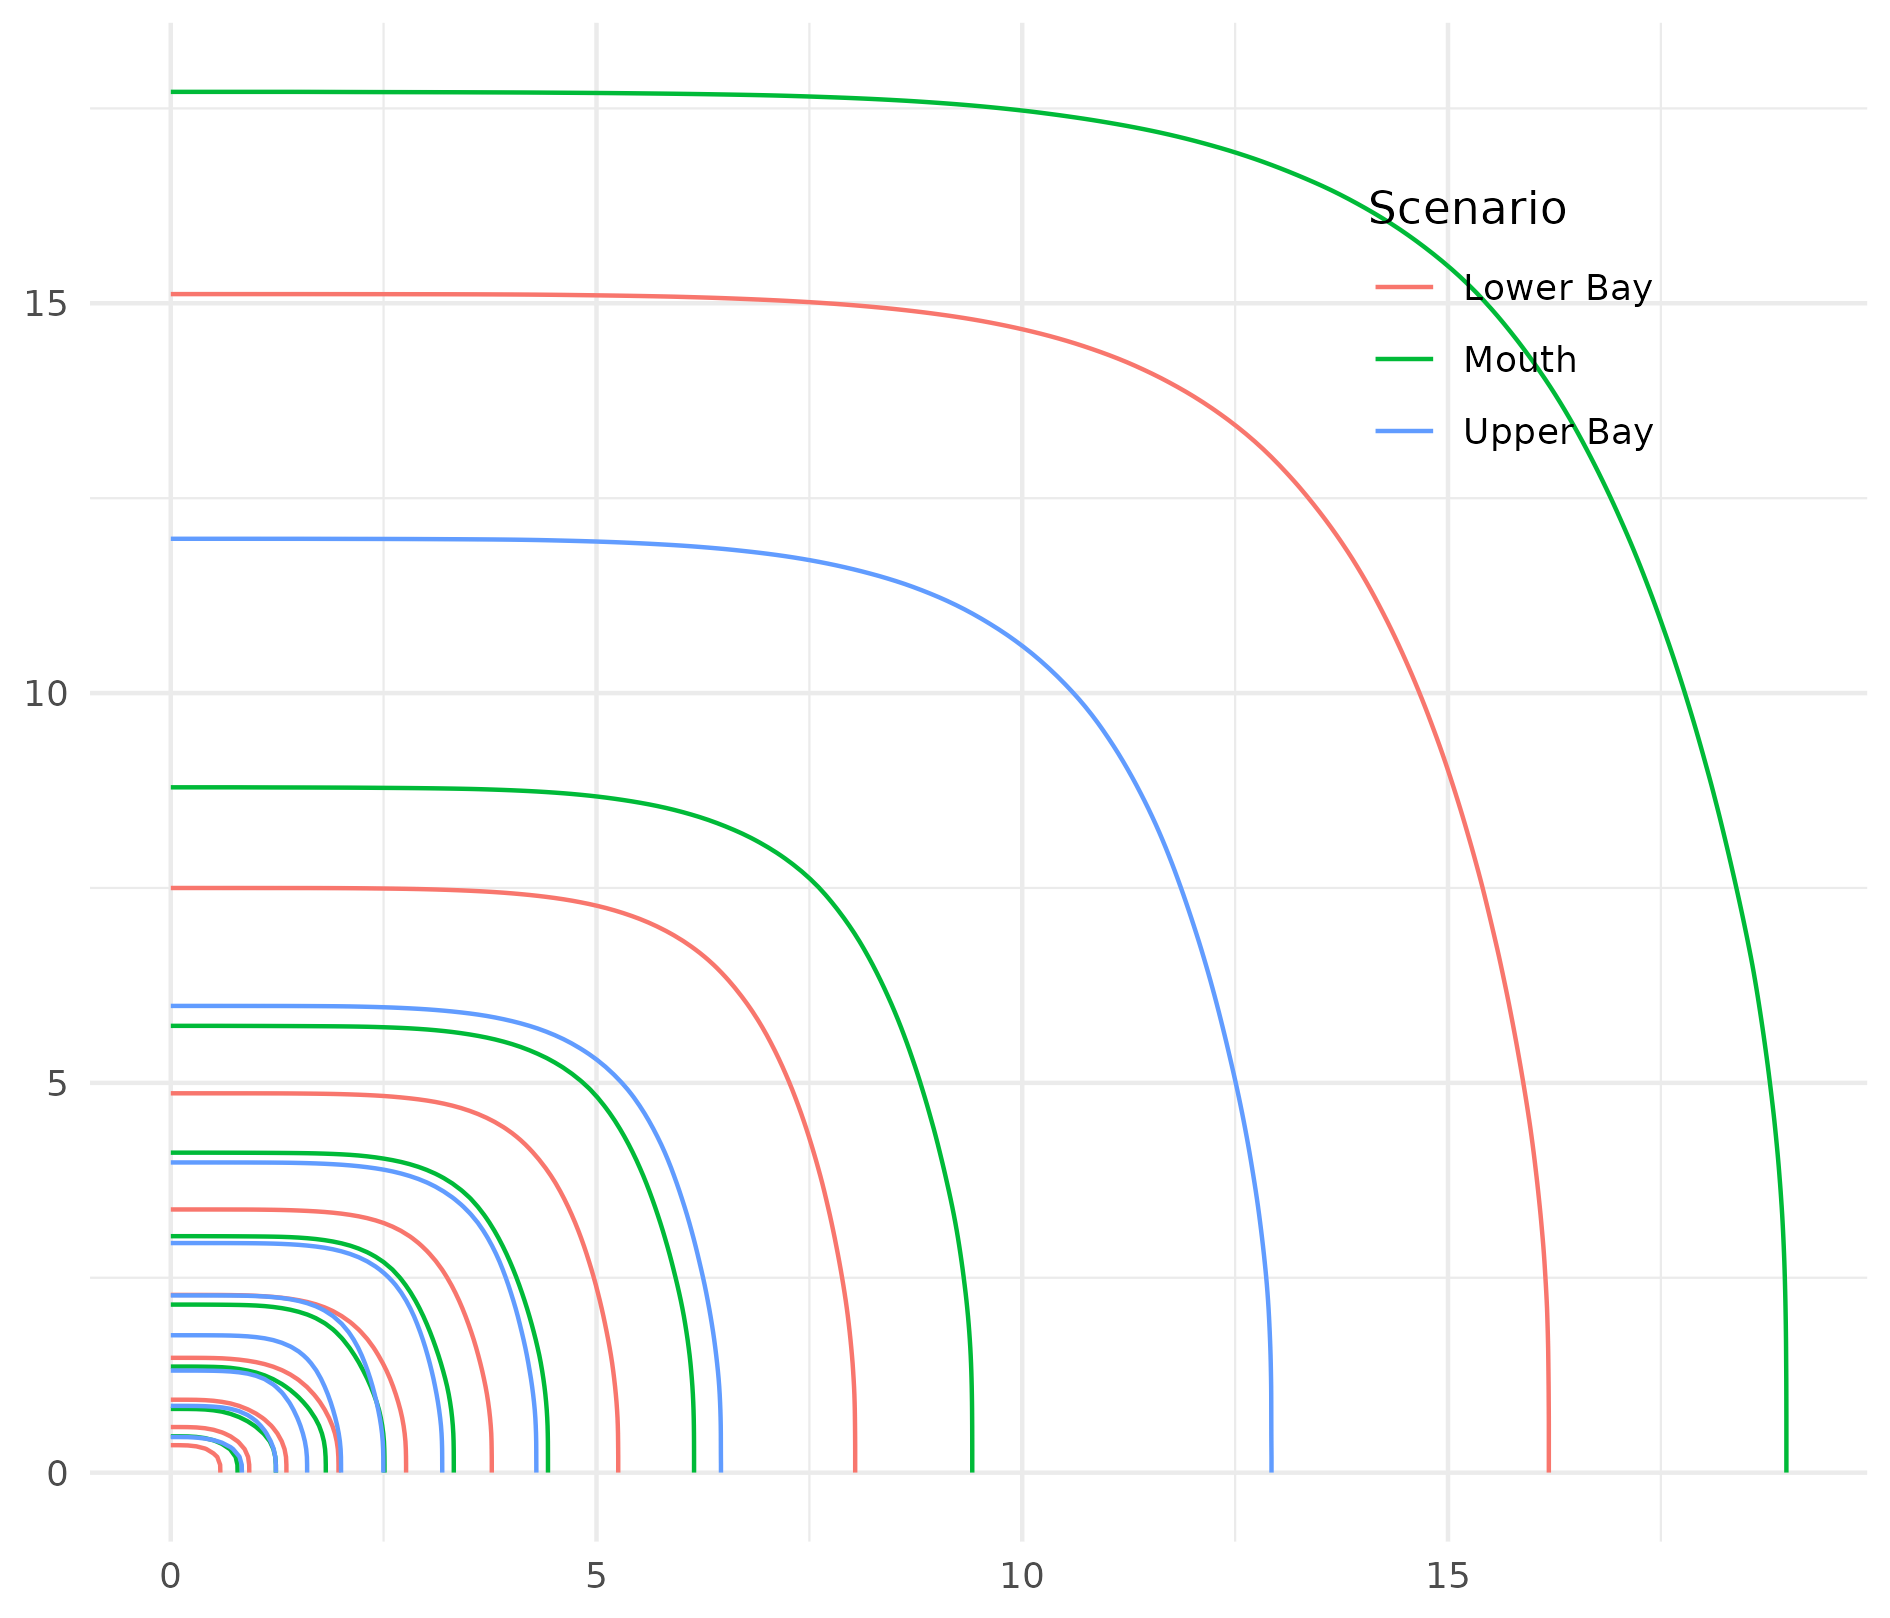
\includegraphics[width=0.3\linewidth]{./plots/condsurv/pia_packer}
    \caption{Conditional Survival Curve (Contour Plot) of flooding at Dover AFB (X) vs Packer Avenue Terminal (Y). 
        \label{fig:condsurv2d:piapacker}
        \makenote{Add plot in real units}}
\end{figure}

Figure~\ref{fig:condsurv2d:piapacker} similarly presents a contour plot of the survival surface between 
    PIA and Packer Avenue terminal. Given the proximity of the locations, we would expect a strong 
    dependence.  That dependence is borne out, as in the contour plot of the survival surface we observe 
    strong convexity.


\makenote{Insert conditional survival curves given threshold under regression model.}

\makenote{insert posterior clustering discussion and pairs plot of cluster assignments of $\bm{\theta}$'s.}

% EOF